\begin{subsectionframemod}{Cross-Domain Few-Shot Object Detection}

    \only<1>{
        \begin{figure}
            \centering
            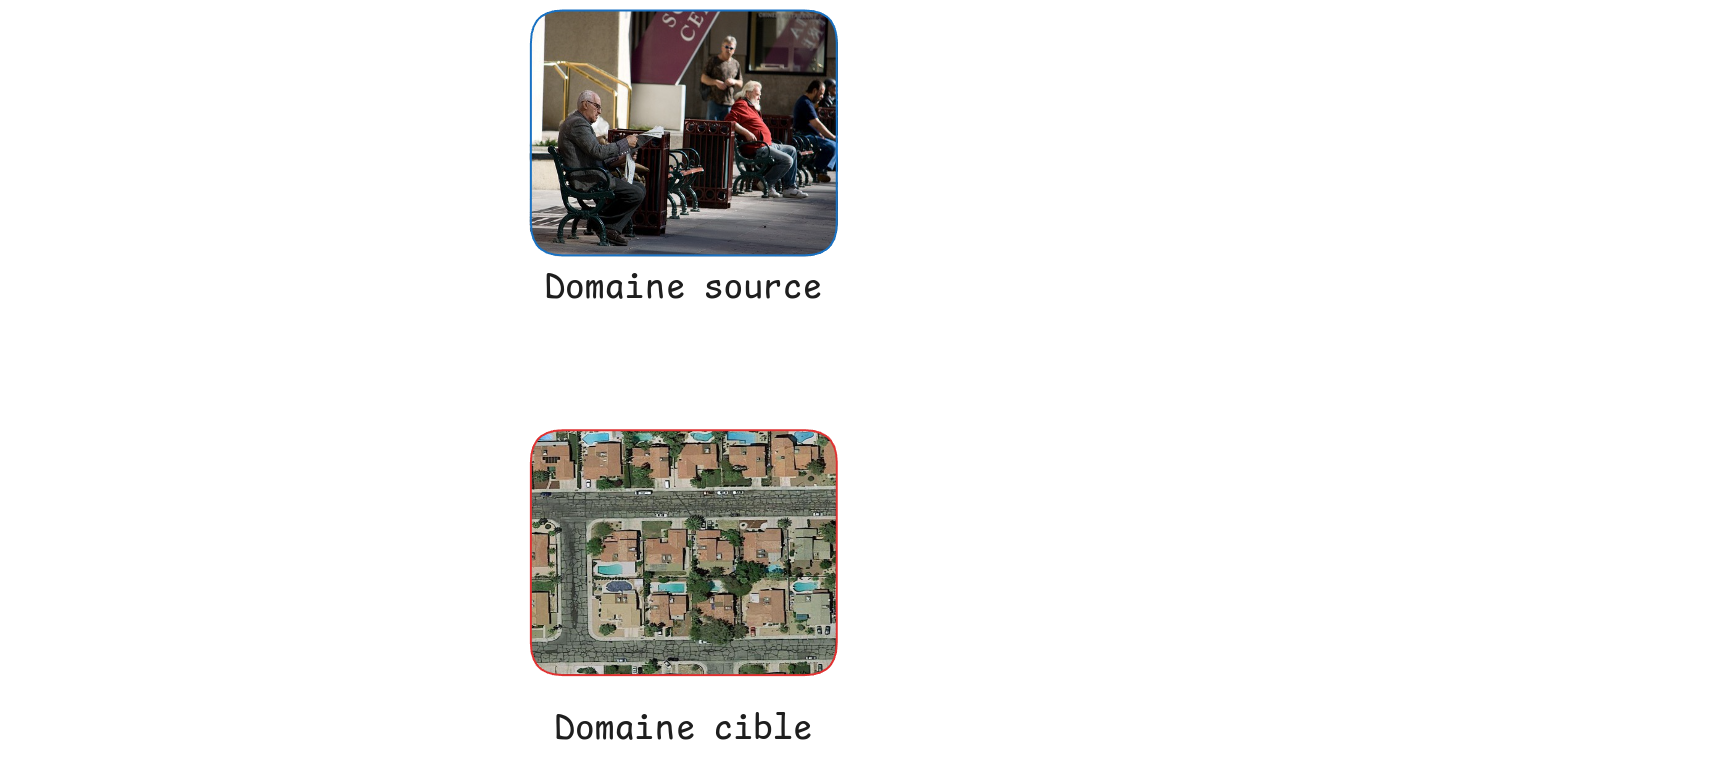
\includegraphics[width=\textwidth]{Figures/cross_domain}
            \caption{Schéma illustrant le cross-domain few-shot, où deux datasets de deux domains distincts sont utilisés pour l'entraînement de base et le fine-tuning.
            Le modèle doit dans ce cas s'adapter à la fois à de nouvelles classes et à de nouvelles images ce qui complexifie la tâche.}
        \end{figure}
    }
    \pause
    \only<2>{
        \begin{figure}
            \centering
            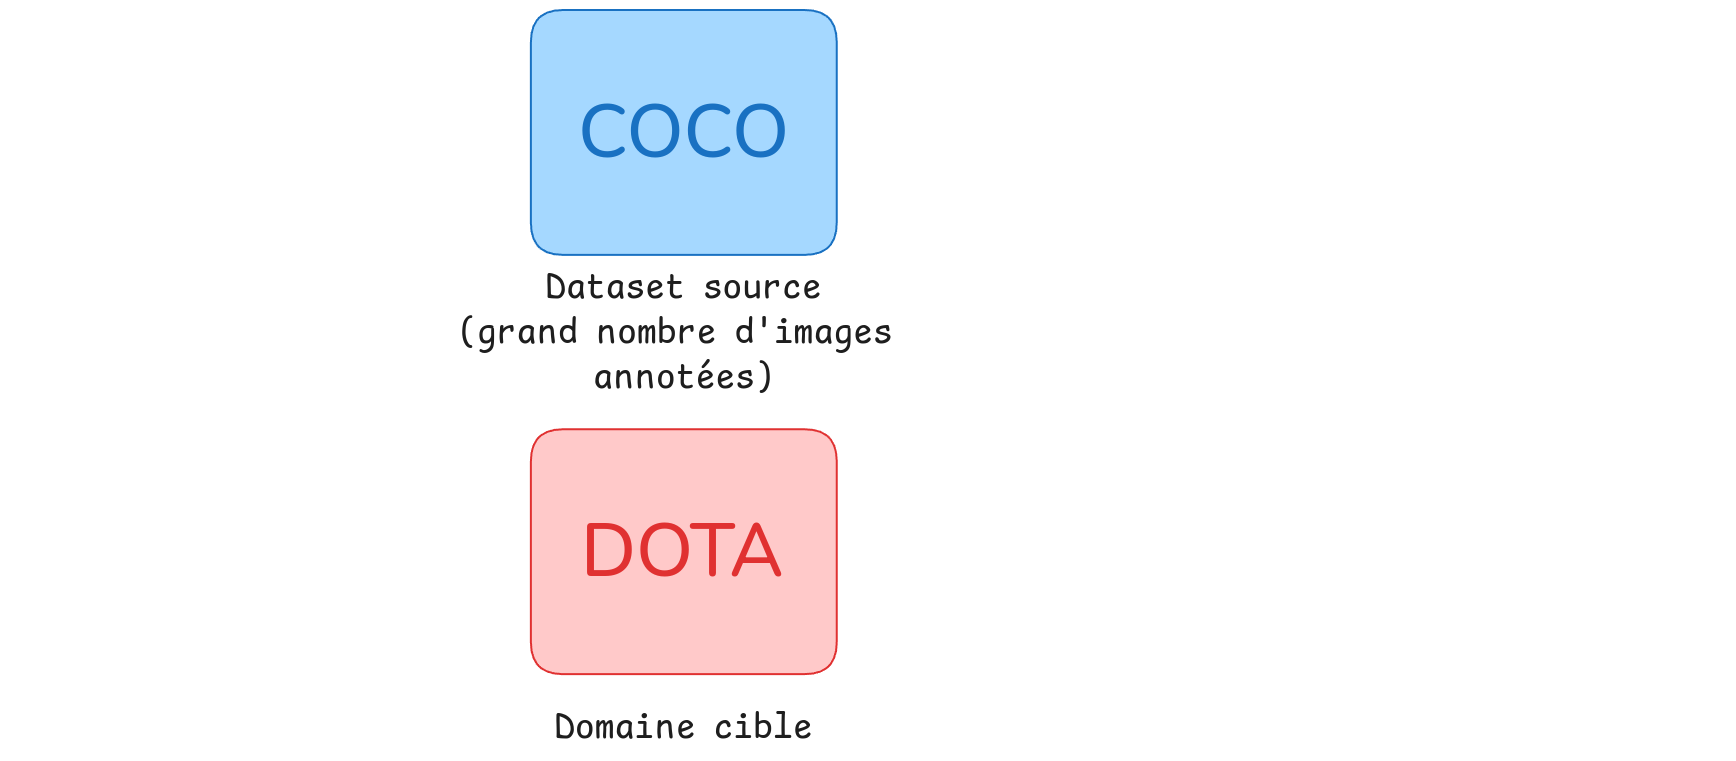
\includegraphics[width=\textwidth]{Figures/cross_domain_0}
            \caption{Schéma illustrant le cross-domain few-shot, où deux datasets de deux domains distincts sont utilisés pour l'entraînement de base et le fine-tuning.
            Le modèle doit dans ce cas s'adapter à la fois à de nouvelles classes et à de nouvelles images ce qui complexifie la tâche.}
        \end{figure}
    }
    \pause
    \only<3>{
        \begin{figure}
            \centering
            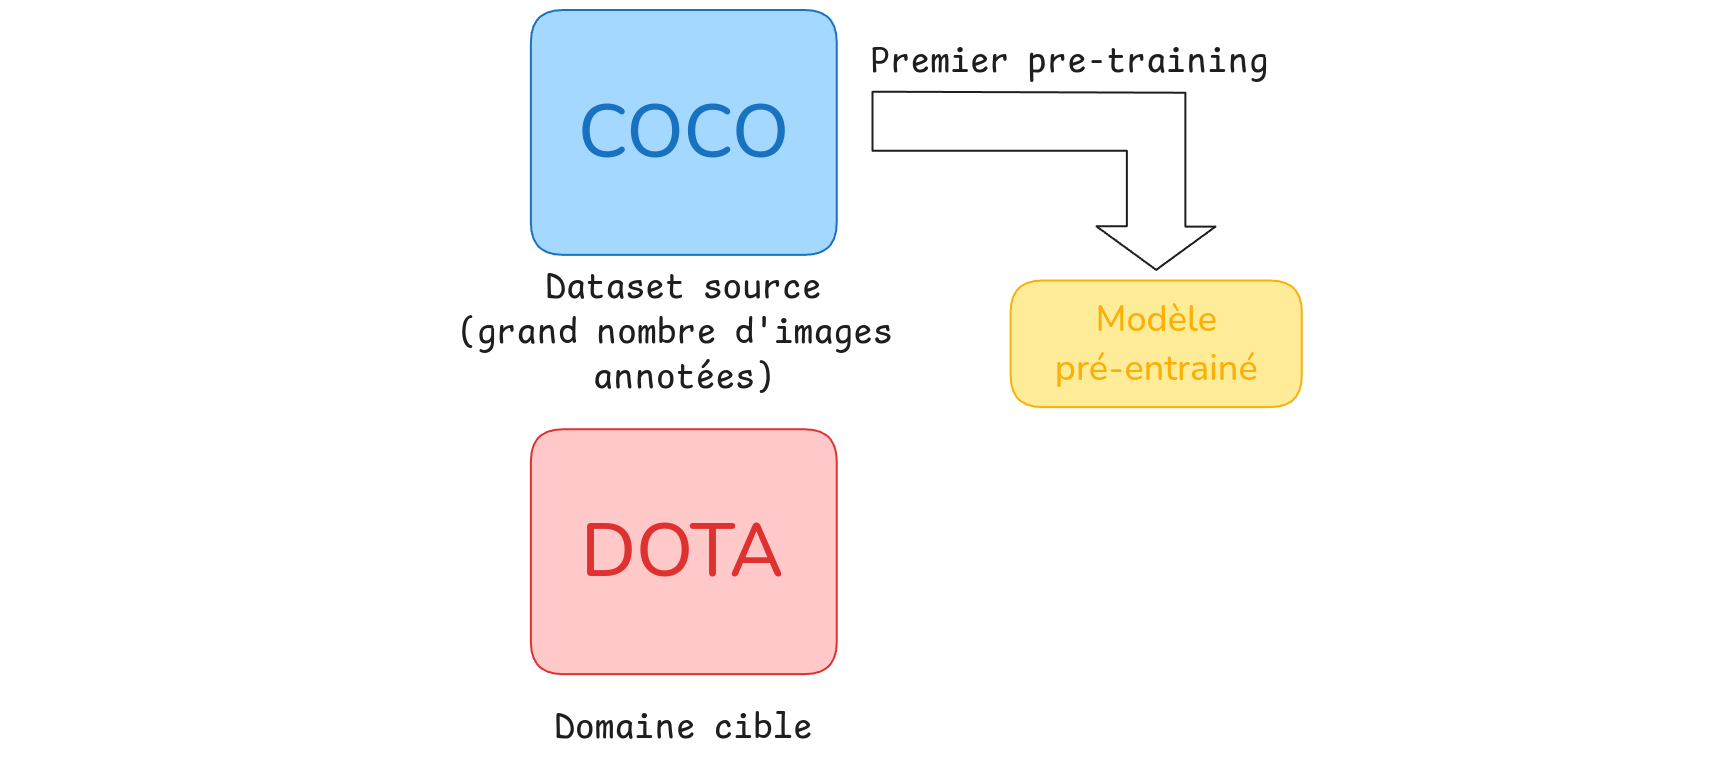
\includegraphics[width=\textwidth]{Figures/cross_domain_1}
            \caption{Schéma illustrant le cross-domain few-shot, où deux datasets de deux domains distincts sont utilisés pour l'entraînement de base et le fine-tuning.
            Le modèle doit dans ce cas s'adapter à la fois à de nouvelles classes et à de nouvelles images ce qui complexifie la tâche.}
        \end{figure}
    }
    \pause
    \only<4>{
        \begin{figure}
            \centering
            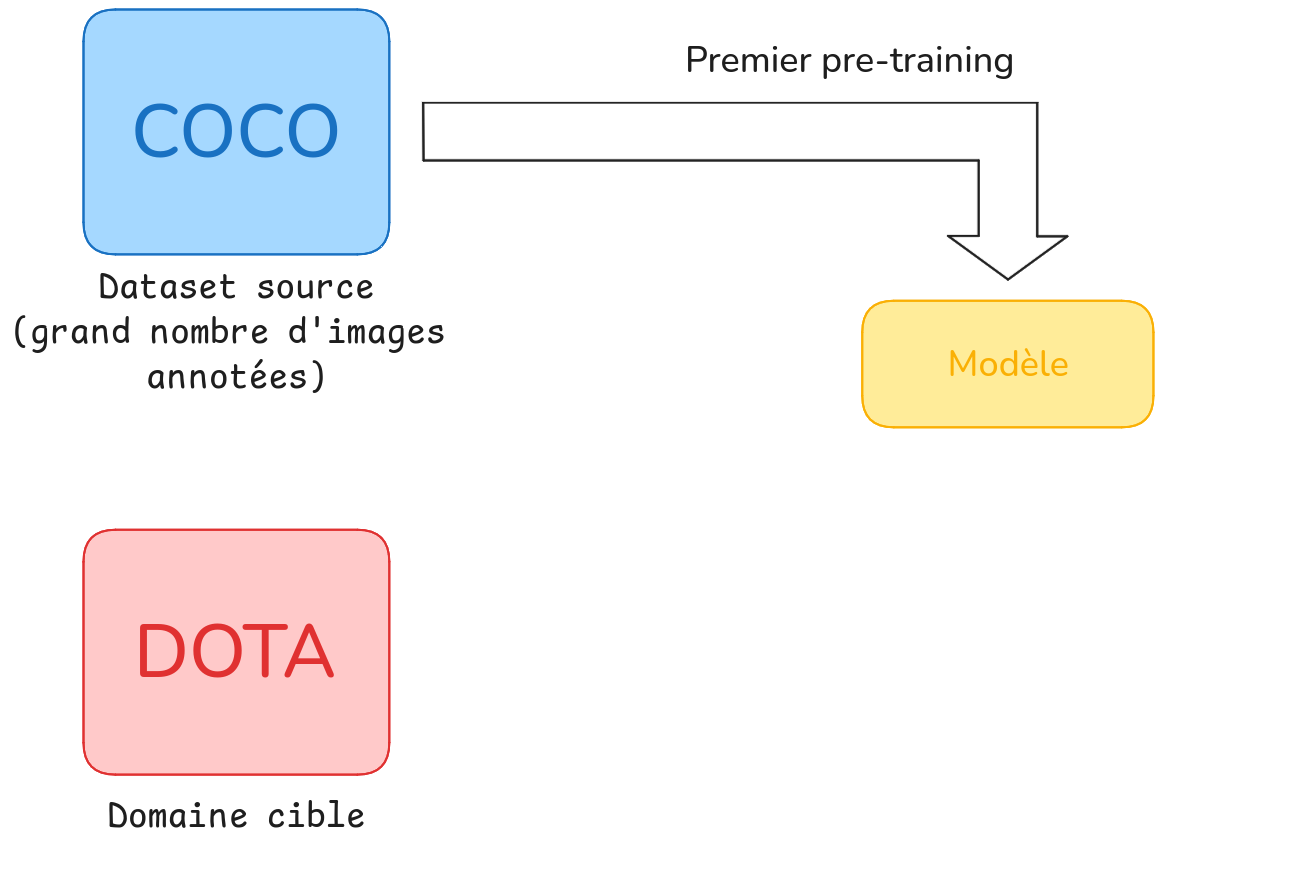
\includegraphics[width=\textwidth]{Figures/cross_domain_2}
            \caption{Schéma illustrant le cross-domain few-shot, où deux datasets de deux domains distincts sont utilisés pour l'entraînement de base et le fine-tuning.
            Le modèle doit dans ce cas s'adapter à la fois à de nouvelles classes et à de nouvelles images ce qui complexifie la tâche.}
        \end{figure}
    }
    \pause
    \only<5>{
        \begin{figure}
            \centering
            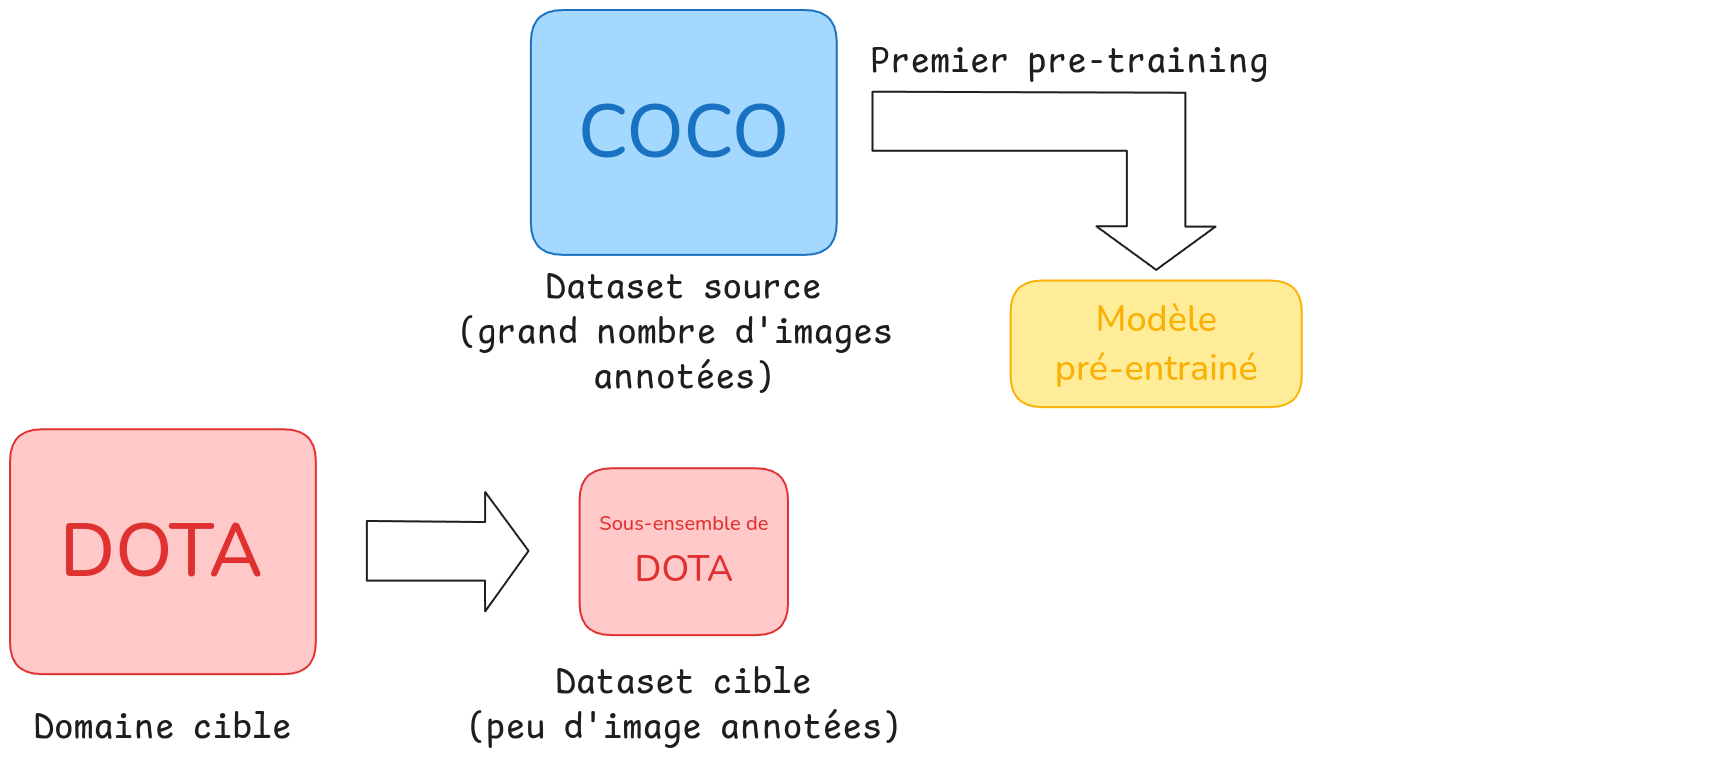
\includegraphics[width=\textwidth]{Figures/cross_domain_3}
            \caption{Schéma illustrant le cross-domain few-shot, où deux datasets de deux domains distincts sont utilisés pour l'entraînement de base et le fine-tuning.
            Le modèle doit dans ce cas s'adapter à la fois à de nouvelles classes et à de nouvelles images ce qui complexifie la tâche.}
        \end{figure}
    }
    \pause
    \only<6>{
        \begin{figure}
            \centering
            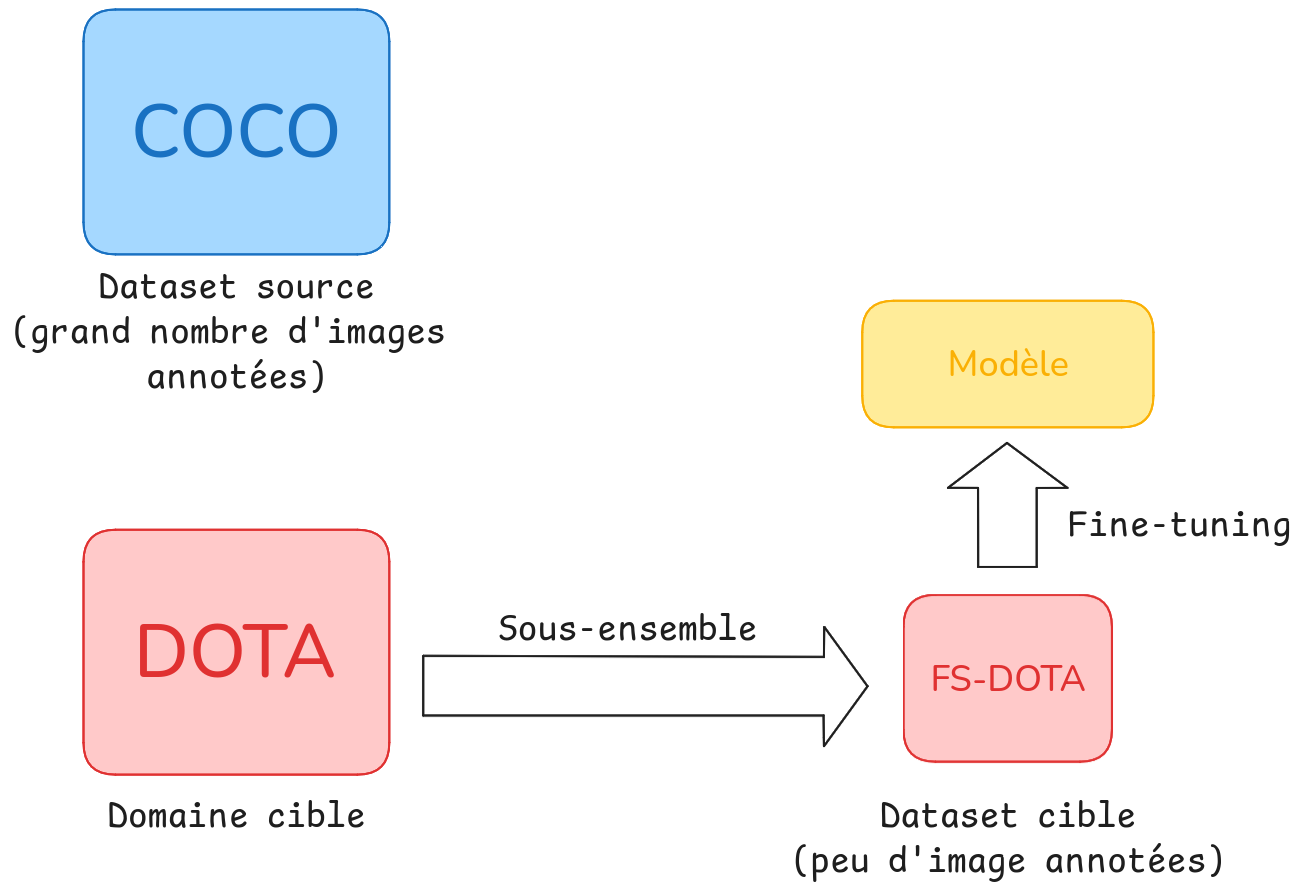
\includegraphics[width=\textwidth]{Figures/cross_domain_4}
            \caption{Schéma illustrant le cross-domain few-shot, où deux datasets de deux domains distincts sont utilisés pour l'entraînement de base et le fine-tuning.
            Le modèle doit dans ce cas s'adapter à la fois à de nouvelles classes et à de nouvelles images ce qui complexifie la tâche.}
        \end{figure}
    }

\end{subsectionframemod}